% % % % % % % % % % % % % % %
\documentclass[11pt]{article}
\usepackage[a4paper, portrait, margin=1in]{geometry}
% % % % % % % % % % % % % % %
\usepackage{graphicx}
\usepackage{listings}
\usepackage{epstopdf}
\usepackage{caption}
\usepackage{svg}
\usepackage{amsmath}
\usepackage{lscape}
\usepackage{multirow}

\newsavebox\IBoxA \newsavebox\IBoxB \newsavebox\IBoxC \newlength\IHeight
\newcommand\TriFig[9]{% Image1 Caption1 Label1 Image2 ...
	\sbox\IBoxA{\includegraphics[width=0.32\textwidth]{#1}}
	\sbox\IBoxB{\includegraphics[width=0.32\textwidth]{#4}}
	\sbox\IBoxC{\includegraphics[width=0.32\textwidth]{#7}}%
	\ifdim\ht\IBoxA>\ht\IBoxB
	\setlength\IHeight{\ht\IBoxB}\else\setlength\IHeight{\ht\IBoxA}\fi%
	\ifdim\ht\IBoxA>\ht\IBoxC
	\setlength\IHeight{\ht\IBoxC}\else\setlength\IHeight{\ht\IBoxA}\fi%
	\ifdim\ht\IBoxB>\ht\IBoxC
	\setlength\IHeight{\ht\IBoxC}\else\setlength\IHeight{\ht\IBoxB}\fi%  
	\begin{figure}[!htb]
		\minipage[t]{0.32\textwidth}\centering
		\includegraphics[height=\IHeight]{#1}
		\caption{#2}\label{#3}
		\endminipage\hfill
		\minipage[t]{0.32\textwidth}\centering
		\includegraphics[height=\IHeight]{#4}
		\caption{#5}\label{#6}
		\endminipage\hfill
		\minipage[t]{0.32\textwidth}\centering
		\includegraphics[height=\IHeight]{#7}
		\caption{#8}\label{#9}
		\endminipage
	\end{figure}%
}

\newcommand\TwoFig[6]{% Image1 Caption1 Label1 Image2 ...
	\sbox\IBoxA{\includegraphics[width=0.5\textwidth]{#1}}
	\sbox\IBoxB{\includegraphics[width=0.5\textwidth]{#4}}%
	\ifdim\ht\IBoxA>\ht\IBoxB
	\setlength\IHeight{\ht\IBoxB}\else\setlength\IHeight{\ht\IBoxA}\fi%
	\begin{figure}[!htb]
		\minipage[t]{0.5\textwidth}\centering
		\includegraphics[height=\IHeight]{#1}
		\caption{#2}\label{#3}
		\endminipage \hfill
		\minipage[t]{0.5\textwidth}\centering
		\includegraphics[height=\IHeight]{#4}
		\caption{#5}\label{#6}
		\endminipage
	\end{figure}%
}


\begin{document}

\title{Advanced Systems Lab (Fall'15) -- Second
Milestone}

\author{Name: \emph{Sandro Huber}\\Legi number: \emph{10-924-777}}

\date{
\vspace{4cm}
\textbf{Grading} \\
\begin{tabular}{|c|c|}
\hline  \textbf{Section} & \textbf{Points} \\ 
\hline  1 &  \\ 
\hline  2 &  \\ 
\hline  3.1 &  \\ 
\hline  3.2 &  \\ 
\hline  4 &  \\ 
\hline  5 &  \\ 
\hline \hline Total & \\
\hline 
\end{tabular} 
}

\maketitle

\newpage

\section{System as One Unit}\label{sec:system-one-unit}

Before coming to the M/M/1 modelling of the system, let's first clarify the notion of request used in this report, since this was not done in the first milestone. In short, a requests is equal to one atomic action of a client, like sending a message or reading all messages of a certain queue. The workload is designed such that, the number of messages in the database stays constant over time. Now that this is explained, let's move to the actual modelling.

The following numbers have been measured in a new stability experiment. For a detailed insight into the configuration and setup, please see section \ref{sec:appendix}. The reason for running a new experiment was the lack of measurements which allow a decent modelling of the system. The following table summarises the measured input parameters for the M/M/1 model:
\begin{center}
	\captionof{table}*{Measured Data} 
	\begin{tabular}{c|c}
		\hline
		Throughput $X$ & 554.94 req/sec \\
		Response Time $R$ & 216.5 ms/req \\
		Queueing Time $Q$ & 142.6 ms/req \\	
		Sleep Time of clients $Z$ & 0.002 ms \\ \hline
	\end{tabular}
\end{center}
When taking this data and putting it into the formulas of the M/M/1 model one ends up with this result:
\begin{center}
	\captionof{table}*{Calculated Data}
	\begin{tabular}{c|c|c}
		\hline
		Arrival Rate $\lambda$ & $\lambda=X$* & $X$ \\
		Service Time $S$ & $S=R-Q$ &71.91 ms/req \\
		Service Rate $\mu$ & $\mu=\frac{1}{S}$ & 13.91 req/sec \\
		Traffic Intensity $\rho$ & $\rho=\frac{\lambda}{\mu}$ & 39.91 \\
		\hline		
	\end{tabular}
\end{center}
\footnotesize*This holds, because the system built is a closed one. This is known, because every client first sends a request into the system and waits until an answer in form of a request comes back. Only then the client proceeds with it's job based on the meaning of the answer. If an answer is lost during transmission or execution the system will automatically take care of this and closes the socket connection to this client, such that it knows an error occured and it has to reconnect if there are still messages not successfully sent yet. This guarantees that no messages are no false positives when logging the throughput.
\normalsize
\newline\newline
Based on the following law:
\begin{equation}
	\text{System is stable}\Leftrightarrow \text{Traffic Intensity} < 1,
\end{equation}
\TwoFig {figures/stability_2/tp.eps} {Throughput of the whole System} {fig:stab2tp}
		{figures/stability_2/rt.eps} {Response Time per Request} {fig:stab2rt}
the system should be heavily unstable. But multiple factors show evidence that this is not the case. First we can have a look at the plots displayed in figures \ref{fig:stab2tp} and \ref{fig:stab2rt}. It's clearly visible that the system is stable. Another factor worth considering in view of this problem is the standard deviation of the throughput and response time which are $20.122$ Req/sec and $7.85$ ms/Req respectively. These two values are identical to $3.626\%$ (throughput) and $3.625\%$ (response time) variation with respect to the corresponding overall mean value, which again indicate a very stable system.

So how to explain then that the traffic intensity $\rho$ $=39.91>1$? The answer lies in the choice of the model. Since the system that was built, internally has a lot of parallelism and works with threads that execute along eachother, the simple M/M/1 model is not able to explain this complex structure and thus fails. The value of the traffic intensity is not random at all though. It is still somewhat connected to the inner structure of the system. Precisely I am talking about the number of database connections, which are constantly 40 during the whole experiment (20 per middleware). In practice this means that on the database, 40 concurrent threads were available which serve concurrently all queries sent from the middlewares. This would perfectly explain the traffic intensity, because when inserting these 40 concurrent threads into the equation: $\rho$ $=\frac{\lambda}{40\mu}=\frac{554.94 \text{ sec/Req}}{40*13.91\text{ Req/sec}}=\frac{554.94 \text{ sec/Req}}{556.4 \text{ Req/sec}}=0.9973<1$. To be sure that all 40 threads on the database are really in use the whole time, we can see if there is queueing happening in the right part of the system. Each request has to go to the database somewhen. The connections are provided through a connection pool. If there are currently no connections available, the request has to wait. In figure \ref{fig:queue_length} we can see that the queue length per middleware is on average of length $38.9$, which makes visible that indeed the database is the bottleneck. These numbers do make sense, because we now can precisely say in which state all the requests are: 40 requests are processed on the database and $2*38.9=77.8$ are waiting for a database connection. Because there were exactly 120 clients online (each one having one open request in the system) we know that we are missing track of $120-40-77.8=2.2$ requests on average. But this makes sense, because there have to be some requests on the way from the database back to the clients and some new ones coming from the clients which did not yet reach the database connection queue.
\begin{figure}
\centering
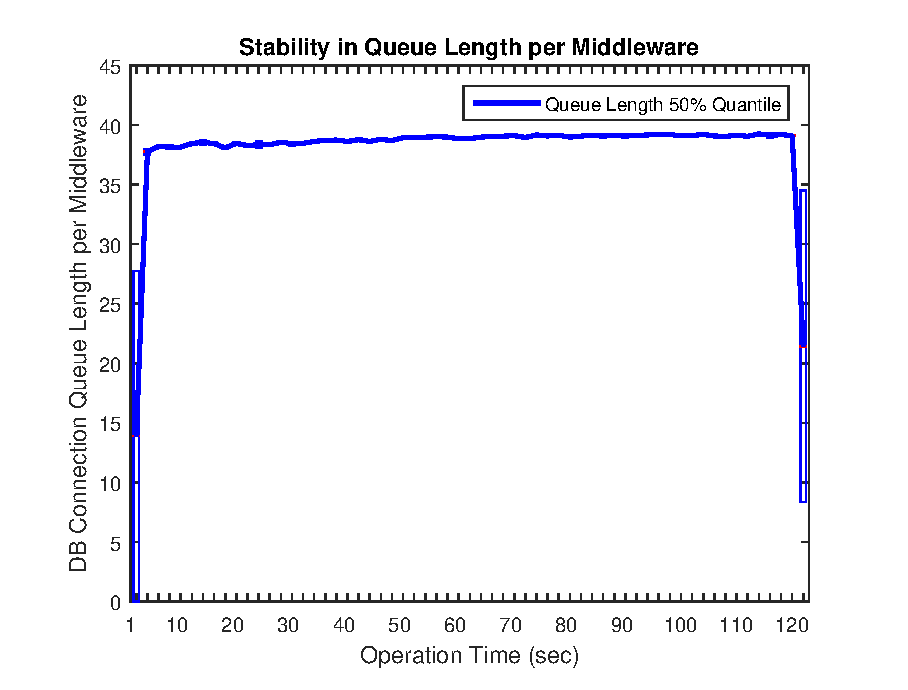
\includegraphics[width=0.6\linewidth]{figures/stability_2/queue_length}
\caption{Queue length in front of DB Connection pool}
\label{fig:queue_length}
\end{figure}

\section{Analysis of System Based on Scalability Data}\label{sec:analysis-scalability}

The scalability of a system has two aspects: it describes the capability of the system to handle an increasing number of requests, but also the possibility of boosting the system performance by adding more modules. It's thus important to include both factors into the analysis. For a detailed description of the experiment setup, please refer to section \ref{sec:appendix}. 

Based on benchmarks evaluated in milestone one, we can assume that the database is the bottleneck in this configuration. As in the book of Raj Jain is written, an M/M/m queue is used to model a multi-server system where jobs for these servers are kept in one queue. In our case, the servers are equal to the threads on the database and the single queue is found as the waiting queue for a database connection on the middleware. It thus make sense to apply an M/M/40 queueing model, because as said, the database provides 40 concurrent connections, and thus, internally runs 40 threads. 

\begin{center}
	\captionof{table}*{M/M/40 Model on Scalability Data for 1 Middleware}
	\begin{tabular}{c|c|c||c|c|c}
		\hline
		& \multicolumn{2}{c||}{Model Parameters} & \multicolumn{3}{c}{Computed and Measured Variables} \\
		\hline
		\#Clients & $\lambda$ (Req/sec) & $\mu$ (Req/sec) & $\rho$ & $\varrho^{*_1}$(\%) & Queue Length$^{*_2}$ \\
		\hline
		10 & 2481.5 & 366.15 & 0.1694 & $2.5783*10^{-13}$ & 0.10\\
		20 & 4773.5 & 341.82 & 0.3491 & 1.15 & 0.20\\
		30 & 7015.5 & 339.42 & 0.5167 & 51.66 & 0.34\\
		40 & 9311.5 & 332.88 & 0.6993 & 69.93 & 0.45\\
		50 & 10346.5 & 303.02 & 0.8536 &85.36 & 0.68\\
		60 & 12302 & 317.06 & 0.9700 & 97.00 & 2.90\\
		70 & 13152 & 329.90 & 0.9967 & 99.67 & 10.66\\
		80 & 13005.5 & 326.25 & 0.9966 & 99.66  & 20.41\\
		90 & 12321 & 308.14 & 0.9996 & 99.96 & 30.84\\
		100 & 13383 & 335.71 & 0.9966 & 99.66 & 38.87\\
		110 & 13013.5 & 326.28 & 0.9971 & 99.71 & 49.56\\
		120 & 12642.5 & 316.59 & 0.9983 & 99.83 & 59.55\\
		\hline		
	\end{tabular}
	\captionof{table}*{$^{*_1}$: Probability of Queueing $^{*_2}$: Measured and averaged per Request}
\end{center}

Let's analyse the outcome of this modelling approach with respect to the previous M/M/1 model. The first improvement visible is the much better fit of the traffic intensity $\rho$. Indeed, the model does now also yield a stable system and thus now mirrors the reality. The model gives also reasonable insights into the probability of when queueing is happening. When we have values of the measured queue length which are $<1$, it means that more requests had an empty queue than requests which had another request actually waiting infront of them already. But the model does also fail in some predictions: For example when wanting to compute the queue length yield by the model via $E[n_q]=\frac{\rho}{\varrho}*(1-\rho)$ the mismatch is immense:

\begin{center}
	\begin{tabular}{c|cccccccccccc}
		\#C & 10 & 20& 30 & 40 & 50 & 60 & 70 & 80 & 90 & 100 & 110 & 120\\\hline
		 & 0.10 & 0.20 & 0.34 & 0.45 & 0.68 & 2.90 & 10.66 & 20.41 & 30.84 & 38.87 & 49.56 & 59.55 \\
		 & 0.00 & 0.00 & 0.00 & 0.00 & 0.00 & 0.00 & 0.03 & 0.14 & 0.30 & 0.48 & 15.14 & $5*10^{15}$\\
	\end{tabular}
\end{center}

The first column shows the measured effective queue lengths on the middleware and the second, the computed one. It is evident that neither the point of the knee, nor the slope of the line does fit onto the data. This is due to the simple M/M/40 modelling approach which does not take into account, that there are effectively two separate components existing in this modelled unit. This leads to the conclusion that this M/M/40 model does fit already quite well onto some initial parameters, but does not lead to further insights afterwards.

The follow-up question to this is, if there are any other models worth trying for the one-middleware setup? The answer is no. Since the whole system is still treated as a black box, there is no other parameter indication besides the one yield by the bottleneck (in our case 40 connections on the database). Additionally it does not make sense to try other ones, when thinking about what context the M/M/40 model was presented: The scalability experiment was run with clients, which tried to send as much as possible. Thus a traffic intensity $\rho$ of close to $1$ does make sense. What happens when trying $m_1<40<m_2$? The M/M/$m_1$ model will yield $\rho>1$, because the parallelism of the database was not fully taken into account and thus the system seems to be unstable. A M/M/$m_2$ model will lead into $\rho<1$, but that's also not optimal, because we already know that the system was operating at its limits. It is therefore not needed to apply another M/M/m model onto the data.

Seeing the resulting throughput of the scalability experiment in figure \ref{fig:scalability_tp} in section \ref{sec:appendix} it's mentionable that having one or two middlewares in action does throughput-wise not make a difference. This should also be expressed in the modelling, when applying the M/M/40 model onto the data of two middlewares. For the sake of redundancy, only the traffic intensity $\rho$ is calculated, to give a brief overview over the fitting quality.

\begin{center}
	\captionof{table}*{M/M/40 Model on Scalability Data for 2 Middlewares}
	\begin{tabular}{c|c|c||c}
		\hline
		& \multicolumn{2}{c||}{Model Parameters} & \multicolumn{1}{c}{Computed and Measured Variables} \\
		\hline
		\#Clients & & & \\
		10  & & & \\
		20 & & & \\
		30 & & & \\
		40 & & & \\
		50 & & & \\
		60 & & & \\
		70 & & & \\
		80 & & & \\
		90 & & & \\
		100 & & & \\
		110 & & & \\
		120 & & & \\
		\hline
	\end{tabular}
\end{center}

\section{Modeling Components as Independent Units}\label{sec:independent-units}

Length: 1-5 pages

In this section you will build M/M/m models of the middleware and the database and explain the characteristics of both. As before, compare them with relevant experimental data and analyse the similarities and differences between models and real behaviour, and link these to specific design decisions in your system.

\subsection{Middleware}\label{sec:mw}
As already explained in the first Milestone, the middleware was built with maximal adaptivity to the current situation in mind. This means that a middleware is able to dynamically allocate resources on demand when either more clients join the system, or in general more requests are generated. To realize this feature, a \textit{cached thread pool} of the \textit{ExecutorService} class has been instantiated to deal with the distribution of requests to threads. The magic behind this class is that it automatically creates and runs threads for each new job, in our case requests, entering the middleware. As shown in the benchmarks for the middleware, this setup allows a very high throughput of around 45'000 requests per second. Since the behaviour of the \textit{cached thread pool} is not fully clear, because one just can't look into its source code, it's necessary to first understand the relationship between the two factors '\#Clients' and '\#Threads'. The number of requests is here not important, because it's not about the throughput (i.e. requests per second), but about the number of requests currently in the system, which is directly correlated to the number of clients.
\newline\underline{Configuration}: This analysis was done on the scalability data. There were one or two middlewares, one database with 40 concurrent connections and two client machines online which provided system access for clients. If two middlewares were online, the clients and database connections were evenly split among both. The clients sent as much as they could, following the load configuration mentioned in milestone 1. Each message had a content of length 200. The number of threads was measured by looping through all available threads and counting those which were in the state \textit{RUNNABLE}.
\newline\underline{Expectation}: The middleware structure is based on a two-step approach: Whenever a new requests enters the middleware, a new thread gets launched which handles the reading, deserialization and database access. When this is completed, this thread shuts down and fires up a second thread that handles the serialization of the answer and sends it back to the corresponding client. So in average there is one thread online per request. Thus we can expect that the equation $\text{'\#Requests in middleware or database'}=\text{'\#Request not in clients'}=\text{'\#Threads'}$ should hold. But in section \ref{sec:system-one-unit} we already saw that only a very small minority of requests is not found in the database or the middleware. With this reasoning we can expect the following behaviour for n clients: $\#Threads=n-\epsilon$, for $\epsilon>0$ and small.
\newline\underline{Reality} (figure \ref{fig:threads}): It's obvious that the mismatch between the measured number of threads and the expectation is serious. What went wrong? The whole analysis was based on the idea of having one thread per request in the middleware or database. But one thing I forgot was the ability of threads to get reused. For example when a request waits for a database connection, its corresponding thread can meanwhile be reused by another request for e.g. deserialization. It therefore holds that  $\text{'\#Requests in middleware or database'}=\text{'\#Request not in clients'}\neq\text{'\#Threads'}$. We still want to correlated the number of clients to the load of the middleware. Although the equation chain does not hold, we still can use its first part, namely $\text{'\#Requests in middleware or database'}=n-\epsilon=\text{'\#Clients'}-\epsilon$, for $\epsilon>0$ and small. By simply counting these requests which currently are processed by either the middleware or the database we end up with a much better fit onto the expectation (figure \ref{fig:refined_mw_load}). We indeed can see that the relation is linear and fulfills the expected bahaviour of $n\approx\text{'\#Requests in middleware or database'}$.

\TwoFig {figures/middleware/threads} {Number of Threads over all\\middlewares under different configurations}
		{fig:threads}
		{figures/middleware/req_vs_clients_on_mw} {Refined load estimation on the middleware} {fig:refined_mw_load}

The figure \ref{fig:refined_mw_load} does verify our assumption of having a linear load-dependent middleware behaviour. This is a problem for modelling, because fitting a single model won't be easy. So let's tackle this problem step by step. First, let's see if there is a model fitting onto every point of the middleware baseline, and in a second step, I try to unite these models into a single one. The first step is done, such that I get more insights into which models fit certain regions of the middleware behaviour and allow easier designing of the single M/M/m model. I quickly repeat the conditions of the middleware baseline:
\newline\underline{Configuration}: The middleware was as isolated as possible, i.e. no database access was made. Two client machines were flooding either one or two middlewares with messages with content length 200. As service time, only the time within the middleware was measured. To apply an M/M/m model, the throughput and service time of the corresponding experiment data were taken. To get an idea of how well different models fit onto the data I did the following: For every point i.e. throughput and response time for $n$ clients, all M/M/m models with m going from 1 to 110 were applied. Because the system was stable in all phases of the experiment, the traffic intensity allows to see how well a model does fit.
\newline\underline{Expectation}: As seen in figure \ref{fig:refined_mw_load}, the load seems to relate linearly to the number of clients, so I have no reason the expect anything else of the models.
\newline\underline{Reality} (figure \ref{fig:load_dependence}): It's clearly visible that the linear trend could be verified also when applying the models. Since the system was stable, but still trying to get as much throughput as possible, a traffic intensity of just below $1$ is expectable. The plot was generated with this assumption in mind. This leads to the basic formula of $|(\rho-1)|^{-1}$, which models the closeness to 1. To have a visually more appealing plot, the final formula reads as $\log(|(\rho-1)|^{-1}+4)$. Additionally to the linear relationship, it's noticeable, that models with higher m's tend to fit more parts of the whole data. This insight is used for the second step, when trying to fit a single model onto the data.

\TwoFig {figures/middleware/load_dependence} {Overview of how well the \\M/M/[1-110] models fit onto the\\ middleware data with respect to the traffic\\ intensity} {fig:load_dependence}
		{figures/middleware/mm95} {Applying the M/M/95 model onto the data of the middleware benchmark} {fig:mm95}

To test a single model onto the middleware, the response time yield by the model and the measured one will be compared. This will give a detailed insight into if and where the model does fit the built system. The approach taken is to model the middleware best when being under maximal load, i.e. when the throughput stagnates, but the response time still grows. This is the case when having 60 clients or more. By examining different models, the best one was found to be the M/M/95 model, which is displayed in figure \ref{fig:mm95}. The model is capable of not only representing the middleware when under maximal load, but also can closely predict the early stages when having a low load. The reason for not having the variance in the plot, is that I already worked with only the 50\% quantile of the data, because the throughput and response time data were logged in different settings (per requests and per second). But to generate a plot like the one seen in figure \ref{fig:mm95}, it's needed to have some sort of common structure. Coming back to the actual plot itself, why is it that exactly the M/M/95 model does the best job, and what is the relation to the real system? As mentioned in the in the first part of this section, threads are reused and thus can handle multiple requests. We saw in figure \ref{fig:threads} that the number of threads when having the maximal throughput, is on average 47 (calculated from the mean values of both settings 1 and 2 MW's). When calculating that the model does yield, that queueing happens with $83.88\%$ on average, we can assume that on average each thread can indeed handle multiple requests, because of the waiting induced by the queueing, but not too much, because of the only very limited time spent in the middleware ($<2.5ms$ on average). Eyeing at the M/M/95 model we can see that a re-usage factor of $\frac{95}{47}=2.02$ requests per thread would not only fit the model perfectly, but also does make sense with respect to the measured data.

\subsection{Database}\label{sec:db}
To find a queueing model for the database one has to take the hardware as well as the software setup into consideration. Let's first start with the hardware specification of the machine used during the experiments, since some of these led to later decisions in the experiment setup itself.

The database was run on a r3.4xlarge machine. By providing 122GiB of RAM it was guaranteed to have small tables fit into the working memory and get good performance. The machine also contained 8 physical CPU's which allows to have 16 parallel threads with hyper threading. By the rule of thumb presented by PostgreSQL itself it holds that the best optimal number of connections is $2*\text{'\#physical cores'}+C$, where $C$ is a constant. In the benchmark it was found that the best performance is reached with 20 concurrent database connections (position of the knee), i.e. the moment before the throughput stops to increase as rapid as in the beginning. Optimality in this context means to have the highest throughput with the least response time. It can be easily viewed in the corresponding figure in milestone 1, that optimal is not equal to maximal. In our case, the maximal throughput is reached when having around 40 database connections. This finding was the reason to run the experiments with 40 database connection if not mentioned otherwise. So from the software point of view we have 40 as an initial guess for the model parameter $m$. When searching through this model space ($m\in[20, 40]$), the best one to come across with respect to the mean squared error between the modelled and measured response time is M/M/30 with $0.0012$ ms of deviation. How is this model connected to the real system? Obviously 30 is exactly between our initial numbers gotten from the hard- and software evaluation, so intuitively it seems to fit. Basically it means, that although 40 threads are running, the performance does not much change with respect to the scenario when having only 30 clients, flooding the database with requests. Eyeing at the throughput plot in milestone 1, we can see that this is indeed the case. The reason for not quite reaching the same throughput as with 40 clients, is because the model does also try to fit onto the the system when it's not fully loaded and thus favours a smaller $m$. It also shows that in our case the rule of thumb does underestimate the power of the system. This can be explained, because the general rule of thumb assumes a default amount of work to be done for every request. In the load used in the experiments we have only one costly (pop message) and four cheap requests. This allows the system to perform better than expected and thus also exceed the lower bound of 20. The M/M/30 model allows to get more insights into how the database performs, for example when the machine starts to reach its performance boundaries.
\TwoFig {figures/database/mm30} {Applying the M/M/30 model onto\\ the data of the database benchmark} {fig:mm40}
		{figures/database/qprob} {Visualisation of the probability of queueing predicted by the M/M/30 model} {fig:qprob}
In figure \ref{fig:qprob} it's shown how the probability of queueing does behave when more clients are spamming requests to the database. The dashed red line indicates the 50\% border. Having data points above this line means, that on average queueing does happen more often than not. Queueing in the context of a database can be interpreted as waiting for a connection, when all connections are currently used. We can not only see that the queueing probability exceeds 50\% at around 30 clients and thus indicates that our choice of model is sound, but also that it's consistent with respect to the throughput measured in the first milestone, because it starts to decrease at around this many clients.
%\begin{figure}
%\centering
%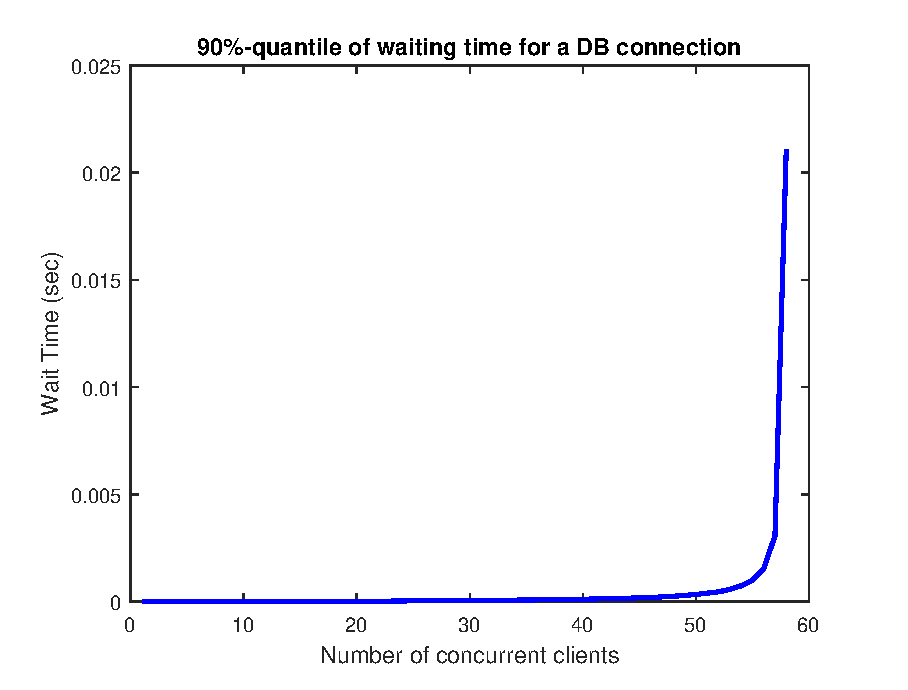
\includegraphics[width=0.7\linewidth]{figures/database/waittime}
%\caption{Estimated wait time for the M/M/30 model}
%\label{fig:waittime}
%\end{figure}

\section{System as Network of Queues}\label{sec:network-of-queues}

Length: 1-4 pages

Based on the outcome of the different modeling efforts from the previous sections, build a comprehensive network of queues model for the whole system. Compare it with experimental data and use the methods discussed in the lecture and the book to provide an in-depth analysis of the behavior. This includes the identification and analysis of bottlenecks in your system.

In the last three section, all important individual system parts have been modelled individually. We can now use this information to try to fit a model when combining the individual parts into a single system. To do this, a network of queues is built.
\newline\underline{Configuration}: To model my system I did choose to take one M/M/30 queue for modelling the database and a M/M/95 queue to simulate the behaviour of the middleware. The clients and the all network delays are packed into a single queue, because neither service time does change with different loads or is dependent on it's position in the system (e.g. before or after the middleware). All of these decision directly follow the results obtained in sections \ref{sec:mw} and \ref{sec:db}. The full setup is shown in figure \ref{fig:networkofqueues}.
\begin{figure}[!htb]
\centering
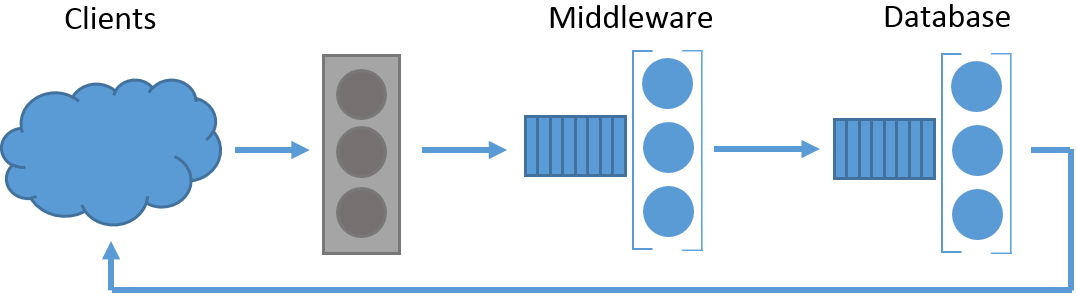
\includegraphics[width=1.0\linewidth]{figures/mva/networkofqueues}
\caption{Schematic setup of the Network of queues to simulate the behaviour of the whole system. The grey box corresponds to the delay center and the other ones to it's corresponding devices.}
\label{fig:networkofqueues}
\end{figure}
To proceed with the modelling, we need to find suitable input parameters for each of the devices. Since each component is modelled as own queue, these number can get extracted out of the baselines computed in the first milestone. The findings are summarized in the following table:

\begin{center}
	\captionof{table}{Fixed Model Parameters} 
	\begin{tabular}{c|c}
		\hline
		Network delays & 0.864723 ms/req \\
		Sleep Time $Z$ & 0.0020 ms/req \\
		Parallelisation factor for Middleware & 95 \\
		Parallelisation factor for Database & 30 \\
		\hline
	\end{tabular}
	\label{tbl:params}
\end{center}

Since we want to work with two load-dependent devices, we need to find a suitable service rate $\mu$ for each one. The problem is that, in contrast to a delay center, the amount of time spent in the device is - as the name suggests - dependent on the load. It thus holds that $\text{constant }C=\mu_{\text{delay denter}}\neq\mu_{\text{load-dependent device}}=f(\text{'\#Clients'})$. To have a suitable approximation of the service time, we used the measurements of the scalability experiment. There, the points for 10, 20, ... 120 clients were collected. It was thus possible to interpolate all missing values to get a fully defined function over the whole spectrum of clients. This was done in \textit{MATLAB} with a call like \textit{interp1(x\_measurements, y\_measurements, x\_estimated, 'pchip');}. It is highly important to account for the parallelisation in each part of the system. Because if a request takes $100$ ms to get processed, the MVA will never give a bigger throughput than $\frac{1}{0.1\text{sec}}=10$ requests per second. It's a good idea to follow an approach proposed in the book of Raj Jain and multiply the number of processed requests by the number of active clients, until either a physical (e.g. physical cores) or software (e.g. number of database connections) boundary is reached. In our case these boundaries were already computed and listed in table \ref{tbl:params}. For example, the multiplication vector for the database looks like $[1,2,3,...,30,30,30,...,30]$, with length of 120. The parameter values listed in table \ref{tbl:params} and the thoughts presented here, lead to the device definition shown in table \ref{tbl:devices}.

\begin{center}
	\captionof{table}{MVA Devices}
	\begin{tabular}{c|c|c|c|c}
		\hline
		System part & Service Time (ms/req) & Type & Parallelisation & \#Visits/req\\
		\hline
		Client + Network & 0.864723 & DC$^{*_1}$ & 1 & 1\\
		Middleware & 0.844386$^{*_3}$ & LDSC$^{*_2}$ & 95 & 1 \\
		Database & 1.327447$^{*_3}$ & LDSC & 30 & 1 \\
		\hline
	\end{tabular}
	\label{tbl:devices}
	\captionof{table}*{$^{*_1}$: Delay center $^{*_2}$: Load-dependent service center \\$^{*_3}$: Example values when having 30 clients}
\end{center}

Based on the device configuration presented in table \ref{tbl:devices} an MVA was performed. To have a fast implementation ready and bea able to evaluate the results properly, a JAVA program was written. The source code is found under $\backslash src\backslash org\backslash asl\backslash mva$.
\newline\underline{Expectation}: As seen in the first milestone, the bottleneck of the whole system was identified as the database. So I expect the MVA to at least give a hint on this behaviour through the utilization output. Since measurements of a real experiment were used as input of the algorithm, the predicted values should come pretty close to the original ones, even thought the interpolation of missing values was only linear. 

\begin{center}
	\captionof{table}{Results of the Mean Value Analysis}
	\begin{tabular}{c|c|c|c|c||c|c}
		\hline
		& \multicolumn{4}{c||}{Computed Values} & \multicolumn{2}{c}{Measured Values} \\
		\hline
		\#Clients & U$_{MW}$ & U$_{DB}$ & X (Req/sec) & R (ms) & X (Req/sec) & R (ms) \\
		\hline
		10 & 0.03 & 0.2 & 2505 & 3.98 & 2482 & 2.76 \\
		20 & 0.06 & 0.36 & 4496 & 4.44 & 4474 & 2.96 \\
		30 & 0.10 & 0.563 & 7004 & 4.28 & 7016 & 2.98 \\
		40 & 0.12 & 0.759 & 9322 & 4.29 & 9312 & 3.04 \\
		50 & 0.14 & 0.86 & 10453 & 4.78 & 10347 & 3.5 \\
		60 & 0.14 & 0.97 & 11180 & 5.36 & 12302 & 3.56 \\
		70 & 0.14 & 0.99 & 11124 & 6.29 & 13152& 4.02 \\
		80 & 0.14 & 0.97 & 11034 & 7.24 & 13006 & 4.81 \\
		90 & 0.14 & 0.99 & 11043 & 8.14 & 12321 & 5.94 \\
		100 & 0.14 & 0.99 & 11010 & 9.1 & 13383 & 6.06 \\
		110 & 0.14 & 0.99 & 10980 & 10.00 & 13014 & 7.06 \\
		120 & 0.14 & 0.99 & 10952 & 10.95 & 12643 & 8.05 \\
		\hline		
	\end{tabular}
	\label{tbl:mva}
\end{center}
\underline{Reality} (table \ref{tbl:mva}): Let's first look at the both columns where the utilization of the middleware and database are listed. It's clearly visible, that the database is fully saturated around 60 clients, whereas the middleware only has to show only a small portion of its capabilities. The position of the knee does indeed also match the one seen in the actual experiment displayed in the figures \ref{fig:stability_tp} and \ref{fig:stability_rt}. From this perspective, the expectation is verified, that the MVA does also mirror the bottleneck behaviour of the database. From the matching of the measured and computed throughput and response time its a bit a different story. The throughput does match very well the measured one until 60 clients are reached. After that point, the throughput does also stagnate, but in a lower region as the one actually measured. Since the system throughput is limited by the database it's possible that the network latency between the middleware and the database was underestimated, and thus the service time of the database was a bit too high, which led to a lower total throughput. It's therefore also not surprising that the overall response time is higher than expected.

The bottleneck is the core optimization point whenever a system is evaluated with respect to performance boosting. To get more insight into it, in the following a bottleneck analysis is done.
\newline\underline{Configuration}: The analysis was done on the scalability data, but there was only one middleware considered (because already one is enough to fully saturate the database). Because of the above mismatch of the response times, the database service time was corrected by $1$ms. This is a big approximation of the real network latency happening between the middleware and the database, because simple pinging between two machines is always dependent on for example the current network usage or machine proximities. This change was needed, because in the original measurements, the database service time was estimated from the middleware, because the inspection of the postgres logs was not doable in time anymore and thus this shortcut had to be taken.
\newline\underline{Expectation}: The database is already in the early stages, i.e. when low numbers of clients are online, the limiting factor in the system. It is therefore reasonable to assume that the actual throughput does follow the asymptotic limit quite closely, when the system if fully saturated. We just saw that this happens at around 60 clients, so there should be a visible come-together of both lines.
\begin{figure}[!htb]
\centering
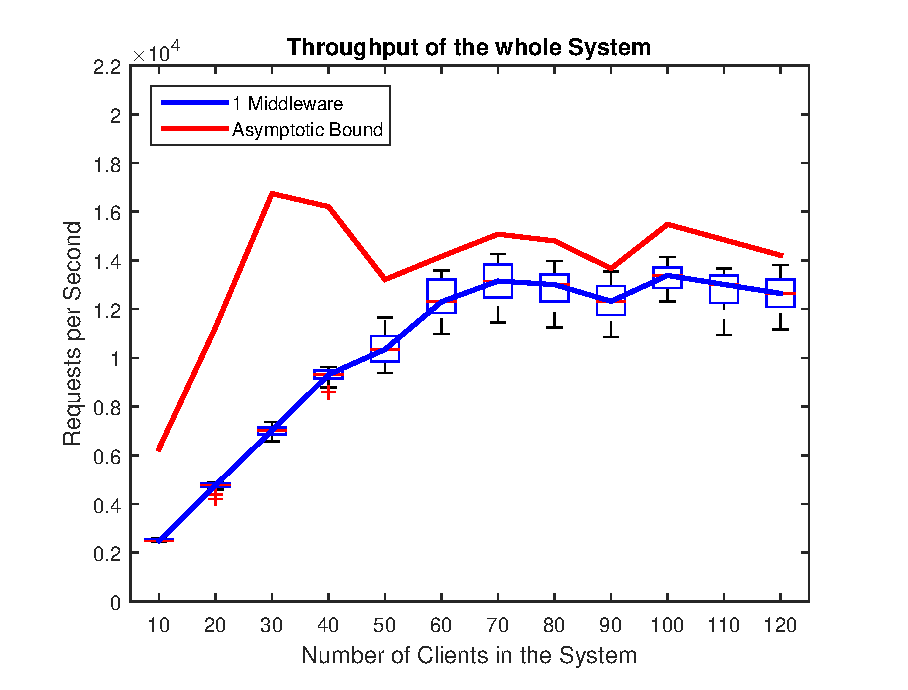
\includegraphics[width=0.7\linewidth]{figures/bottleneck/bottleneck}
\caption{Asymptotic behaviour of the throughput when limited by the database as bottleneck.}
\label{fig:bottleneck}
\end{figure}
\newline\underline{Reality} (figure \ref{fig:bottleneck}): Despite the coarse approximation of the network, it's possible to get some valuable information of the graph. First of all, the curves do show a very similar behaviour from the moment on, where the system is saturated, i.e. when the database starts to get overwhelmed by the amount of requests. When the system is only accessed by a low number of clients, the per-request service time is lower because there is no congestion happening between the different database threads. At 30 clients, this behaviour suddenly changes and the database starts to get the limiting factor of the whole system, visible by the shrinking distance between the two lines. That this break happens at 30 clients is not surprising at all, since in section \ref{sec:db} we concluded that the database is best represented by a M/M/30 queue. The discrepancy between the curve in the saturated region is explained by the rough approximation of the network latency between the middleware and database, the middleware service time which also introduces some milliseconds and the whole network between the clients and the middleware. This reasoning thus allows to confirm that the database is indeed the bottleneck.

In case of wanting the system to perform better, the database would be the part where improvements are directly measurable. Having a better (i.e. more threads, more RAM, more CPU's, ect...) database the red line in figure \ref{fig:bottleneck} would not only be generally higher, but also the two points currently located at 30 and 60 clients could possibly move more towards the right. In practice this would mean that the overall system performance can handle more clients before it is saturated (assuming it is still the database is still the limiting system part).

\section{Interactive Law Verification}\label{sec:interactive-law}

Length: 1-2 pages

Check the validity of all experiments from milestone 1 using the interactive law. Analyze the results and explain them in detail.

mw baseline: with 1 cm interactive law does not fit the line, because with that setup the system was not closed? the client was not able to bring enough reqeuests, and started to block itself. thats way less throughput was registered and higher response times are expected, but not measured, because the middleware was not at it's limits yet.

stability: discrepancy at the beginning due to the high think time used to setup clients.

2k verification:

\begin{tabular}{c|c|c||c|c}
	TP(Req/s) & RT(ms) & IRL(ms) & Abs. Difference(ms) & Percentual Difference(\%) \\
	\hline
	12427 & 5.12 & 4.83 & 0.29 & 5.66 \\
	14707 & 3.87 & 4.08 & 0.21 & 5.43 \\
	11859 & 4.84 & 5.06 & 0.22 & 4.55 \\
	16133 & 3.66 & 3.72 & 0.06 & 1.64 \\
	12413 & 9.98 & 9.67 & 0.31 & 3.11 \\
	18233 & 7.07 & 6.58 & 0.49 & 6.93 \\
	13238 & 9.14 & 9.06 & 0.08 & 0.88 \\
	16428 & 6.97 & 7.30 & 0.33 & 4.73 \\
	13488 & 4.69 & 4.45 & 0.24 & 5.12 \\
	15954 & 3.87 & 3.76 & 0.11 & 2.84 \\
	12289 & 4.94 & 4.88 & 0.06 & 1.21 \\
	15855 & 4.19 & 3.78 & 0.41 & 9.76 \\
	13017 & 9.16 & 9.22 & 0.06 & 0.66 \\
	17701 & 6.57 & 6.78 & 0.21 & 3.20 \\
	13054 & 9.31 & 9.19 & 0.12 & 1.29 \\
	17619 & 6.73 & 6.81 & 0.08 & 1.19 \\
	\hline  
	&&& avg: 0.21 & avg: 3.64 \\
	\hline  
\end{tabular}

\TwoFig {figures/interactive_law/db_baseline} {IL on DB Baseline} {}
		{figures/interactive_law/db_data_baseline} {IL on DB Data Baseline} {}

\TwoFig {figures/interactive_law/db_data_baseline_third_index} {IL on DB Data Baseline with 3rd Index} {}
		{figures/interactive_law/mw_baseline} {IL on MW Baseline} {}
		
\TwoFig {figures/interactive_law/client_baseline} {IL on Client Baseline} {}
		{figures/interactive_law/stability} {IL on Stability} {}
		
\TwoFig {figures/interactive_law/rt_1cm} {IL on Client Baseline} {}
		{figures/interactive_law/rt_2cm} {IL on Stability} {}

\section*{Appendix: Repeated Experiments}\label{sec:appendix}

As told in section \ref{sec:system-one-unit}, the measured data from milestone one was not sufficient to do a modelling of the system. Thus, the two experiments stability and scalability were rerun. Let's first look at the stability experiment. Since this experiment did not change in setup, configuration or evaluation, here, just the main facts are repeated for locality and practicality reasons.
\newline\underline{Configuration}: The stability trace was run with one database, two middlewares and two client machines, each providing 60 clients which send requests with a content length of 200. In total, 40 database connections were distributed. Both of the middlewares got 20 each. The database was initially filled with 300'000 messages to simulate a more real-world behaviour. In contrast to the long stability trace done in the first milestone, this experiment was only run for 120 seconds. This is ok, because in the first experiment the system was already stable after 10 seconds and thus it seemed enough to just get 100 seconds of valid stable data (when ignoring the first and last 10 seconds because of warm-up and cooldown phases).
\newline\underline{Expectation}: The system was already confirmed to be able to run stably under this configuration, so there is no reason to expect something else.
\newline\underline{Reality} (figures \ref{fig:stab2tp} and \ref{fig:stab2rt}): When comparing the results from this stability trace and the one done in milestone one, it's evident that there is a big mismatch with respect to throughput and response time. There was a constant shift down to $56\%$ of the throughput. This can be explained by either more network usage by other customers or a bigger distance between the machines. The important fact here though is, that the system is indeed stable again and thus is valid as input data for this modelling task. Sadly because of limited time and money budget I was not able to run the experiment again and thus had to work with this data. For the sake of not repeating plots or data, the interactive law verification is already shown in figure \ref{fig:stab2rt}.

As mentioned, the second experiment repeated for this milestone was the scalability run, let's go over its setup and outcome, too. The scalability experiment was not run explicitly enough in the first milestone and with the focus ond the wrong factors. This time the main factors numbers of middlewares and clients were closely analysed.
\newline\underline{Configuration}: The goal of this experiment is to find out the impact of how different system sizes do influence the overall performance. To achieve this, either one or two middlewares were active, serving in total 10, up to 120 clients. Each of these clients followed the same workload procedure and sent messages with a content length of 200. Since it was already clear that the best configuration for the system includes 40 concurrent database connections this was fixed throughout the whole experiment. If there were two middlewares running, both got 20 connections for their internal connection pool. 
\newline\underline{Expectation}: In the first milestone the maximal throughput yield a throughput knee with 60 clients, after that the throughput stagnates and only the response time per requests grows. It thus can be expected, that this behaviour should also be visible in this experiment. Estimating the number of requests per second is a bit tricky, since in the previous experiment there were some inconsistencies with respect to data earlier measured. It's known, that the database as limiting system piece maximally allows $\approx$ 20'000 requests per second. Since the overall system performance seems to be lower, the expected throughput lies at around $\approx$ 11'000. Because of the database limitation there should be no difference in throughput between the one or two middlewares setup.
\TwoFig {figures/scalability/tp} {Throughput over the\\ whole system.} {fig:scalability_tp}
		{figures/scalability/rt} {Response time over the whole system.} {fig:scalability_rt}	
\newline\underline{Reality} (figures \ref{fig:scalability_tp} and \ref{fig:scalability_rt}): It's great, that the expectation could be verified, that the number of middlewares is not important, because the database cuts off earlier. The predicted knee at 60 clients is also visible and makes the experiment a success. The maximal number of requests per second was underestimated though. In the previous experiment, the database was not empty as in this one, so there are probably other hidden factors which influence this drop down. But overall the behaviour is the same as expected and is usable for the upcoming modelling tasks. For convenience, the interactive law is already plotted in figure \ref{fig:stability_rt}.

\end{document}
